% This must be in the first 5 lines to tell arXiv to use pdfLaTeX, which is strongly recommended.
\pdfoutput=1
% In particular, the hyperref package requires pdfLaTeX in order to break URLs across lines.

\documentclass[11pt]{article}

% Change "review" to "final" to generate the final (sometimes called camera-ready) version.
% Change to "preprint" to generate a non-anonymous version with page numbers.
\usepackage[final]{acl}

% Standard package includes
\usepackage{times}
\usepackage{latexsym}

% For proper rendering and hyphenation of words containing Latin characters (including in bib files)
\usepackage[T1]{fontenc}
% For Vietnamese characters
% \usepackage[T5]{fontenc}
% See https://www.latex-project.org/help/documentation/encguide.pdf for other character sets

% This assumes your files are encoded as UTF8
\usepackage[utf8]{inputenc}

% This is not strictly necessary, and may be commented out,
% but it will improve the layout of the manuscript,
% and will typically save some space.
\usepackage{microtype}

% This is also not strictly necessary, and may be commented out.
% However, it will improve the aesthetics of text in
% the typewriter font.
\usepackage{inconsolata}

%Including images in your LaTeX document requires adding
%additional package(s)
\usepackage{graphicx}

% \usepackage{multirow}

% If the title and author information does not fit in the area allocated, uncomment the following
%
%\setlength\titlebox{<dim>}
%
% and set <dim> to something 5cm or larger.

\title{iShumei-Chinchunmei at SemEval-2025 Task 4: A Multi-Task Unlearning Approach Integrating Data Augmentation and Gradient Interference}

% Author information can be set in various styles:
% For several authors from the same institution:
% \author{Author 1 \and ... \and Author n \\
%         Address line \\ ... \\ Address line}
% if the names do not fit well on one line use
%         Author 1 \\ {\bf Author 2} \\ ... \\ {\bf Author n} \\
% For authors from different institutions:
% \author{Author 1 \\ Address line \\  ... \\ Address line
%         \And  ... \And
%         Author n \\ Address line \\ ... \\ Address line}
% To start a separate ``row'' of authors use \AND, as in
% \author{Author 1 \\ Address line \\  ... \\ Address line
%         \AND
%         Author 2 \\ Address line \\ ... \\ Address line \And
%         Author 3 \\ Address line \\ ... \\ Address line}

\author{
  Yujian Sun\textsuperscript{1},
  Tian Li\textsuperscript{2}
\\
  \textsuperscript{1}Shumei AI Research Institute, Beijing, China\\
  \textsuperscript{2}School of Computing, Newcastle University, Newcastle upon Tyne, UK
\\
  \texttt{sunyujian@ishumei.com}\\
  \texttt{t.li56@newcastle.ac.uk}
}

%\author{
%  \textbf{First Author\textsuperscript{1}},
%  \textbf{Second Author\textsuperscript{1,2}},
%  \textbf{Third T. Author\textsuperscript{1}},
%  \textbf{Fourth Author\textsuperscript{1}},
%\\
%  \textbf{Fifth Author\textsuperscript{1,2}},
%  \textbf{Sixth Author\textsuperscript{1}},
%  \textbf{Seventh Author\textsuperscript{1}},
%  \textbf{Eighth Author \textsuperscript{1,2,3,4}},
%\\
%  \textbf{Ninth Author\textsuperscript{1}},
%  \textbf{Tenth Author\textsuperscript{1}},
%  \textbf{Eleventh E. Author\textsuperscript{1,2,3,4,5}},
%  \textbf{Twelfth Author\textsuperscript{1}},
%\\
%  \textbf{Thirteenth Author\textsuperscript{3}},
%  \textbf{Fourteenth F. Author\textsuperscript{2,4}},
%  \textbf{Fifteenth Author\textsuperscript{1}},
%  \textbf{Sixteenth Author\textsuperscript{1}},
%\\
%  \textbf{Seventeenth S. Author\textsuperscript{4,5}},
%  \textbf{Eighteenth Author\textsuperscript{3,4}},
%  \textbf{Nineteenth N. Author\textsuperscript{2,5}},
%  \textbf{Twentieth Author\textsuperscript{1}}
%\\
%\\
%  \textsuperscript{1}Affiliation 1,
%  \textsuperscript{2}Affiliation 2,
%  \textsuperscript{3}Affiliation 3,
%  \textsuperscript{4}Affiliation 4,
%  \textsuperscript{5}Affiliation 5
%\\
%  \small{
%    \textbf{Correspondence:} \href{mailto:email@domain}{email@domain}
%  }
%}

\begin{document}
\maketitle
\begin{abstract}

%本文描述了我们在SemEval-2025任务4中的解决方案,描述了一种用于解决有限资源下用于大模型unlearning sensitive datasets的监督微调方法。我们的方法集成了多任务学习、梯度干扰以及数据增强。通过这种方法,我们的方法在部分任务中表现优异。此外,通过消融实验和结果分析我们发现了单纯的监督微调在unlearning sensitive datasets in LLMs中可能存在的一些问题。

This paper presents our solution for SemEval-2025 Task 4, introducing a supervised fine-tuning method for unlearning sensitive data in large language models (LLMs) under resource constraints. Our approach combines multi-task learning, gradient interference, and data augmentation, achieving promising results across several tasks. Additionally, through extensive ablation experiments and detailed result analysis, we identify potential issues that arise when relying solely on supervised fine-tuning for unlearning sensitive data.
\end{abstract}

\section{Introduction}

%大语言模型(LLMs)在自然语言理解和生成方面表现出了卓越的性能。然而,由于它们是基于大量数据进行训练的,它们可能会无意中保留并重复敏感信息,从而引发关于隐私和合规性的严重担忧。SemEval-2025任务4:“从大语言模型中遗忘敏感内容”旨在旨在通过开发一个全面的评估挑战来弥补缺乏强大的评估框架来评估这些反学习策略的准确性的问题。对于确保伦理的AI部署并符合隐私法规至关重要。该任务以英语进行,评估将考虑任务特定的重复率、成员推断攻击(MIA)得分和MMLU基准性能,以衡量模型在遗忘指定内容的同时,保持其更广泛的语言和推理能力的有效性。

%八股文
%第一段讲任务是什么,存在什么问题,比赛为了解决什么问题。介绍数据集,这份数据集提出、鼓励研究人员推动unlearning的贡献。
%第二段,我们参加了这次比赛,在比赛中我们干了个什么事,要写一个原因,我们尝试了一些基于梯度和机遇数据增强的方案,为什么我们采用这些方案。我们做了什么适配,对梯度做了什么改动。high leval
%我们的贡献如下:1.2.3.,
%1.第一个一定是用了什么技术,全称+简单做法。
%2.高角度的high level的增益有什么,通过详细的实验,我们发现xxx对我们最终的效果有贡献,这揭示了xxxx的有效性。
%3.要不要补充更多的贡献,我们最终的榜单排在第几。


Large Language Models (LLMs) have demonstrated remarkable performance in natural language understanding and generation. However, as they are trained on vast amounts of data, they may unintentionally retain and regurgitate sensitive information, posing serious concerns regarding privacy and compliance. 
SemEval-2025 Task 4: "Unlearning Sensitive Content from Large Language Models"
(\citep{ramakrishna2025lumellmunlearningmultitask})
seeks to address the lack of a robust evaluation framework for assessing the accuracy of unlearning strategies by providing a comprehensive evaluation challenge. 
This task is crucial for ensuring the ethical deployment of AI and compliance with privacy regulations.
Conducted in English, the evaluation will consider metrics such as task-specific regurgitation rates, Membership Inference Attack (MIA) scores, and MMLU benchmark performance, to measure how effectively the model forgets specified content while retaining its broader language understanding and reasoning abilities.\par

%我们的系统采用了多任务学习方法,并结合梯度干扰技术和数据增强来改善反学习过程。具体来说,我们引入了多个训练目标,以控制模型如何处理保留数据和遗忘数据。对于需要保留的数据,我们应用监督微调(Supervised Fine-Tuning,SFT)损失,确保模型保持其一般知识。对于必须遗忘的数据,我们采用了梯度干扰,一种灵感来源于梯度上升的Gradient Ascent损失函数。此外,我们也对将类似I don't know的文本替换遗忘数据的输出文本的方案进行了尝试。为了增强模型在不同输入长度和上下文中的鲁棒性,我们应用数据增强技术,将答案拆分为句子并重新组合,生成多样化的训练实例。这一策略确保模型在有效学习遗忘内容的同时,保持其在非敏感数据上的表现。

Our system adopts a multi-task learning approach combined with gradient interference techniques and data augmentation to enhance the unlearning process. Specifically, we introduce multiple training objectives to regulate how the model handles retained and forgotten data. 
For data that must be retained, we apply Supervised Fine-Tuning (SFT) loss to ensure the model preserves its general knowledge. 
For data that needs to be forgotten, we implement gradient interference, inspired by the Gradient Ascent loss function. Additionally, we experiment with replacing the outputs of forgotten data with negative responses resembling  "I don’t know." (\citet{choi2024snap};\citet{shi2024ulmr}) 
To improve the model's robustness across varying input lengths and contexts, we apply data augmentation techniques, such as breaking answers into sentences and recombining them to generate diverse training instances. 
This strategy ensures that the model effectively learns which content to forget while maintaining its performance on non-sensitive data.

%我们的系统在SemEval-2025任务4中,基于7B模型的效果排名第五。实验结果表明,我们的方法能够在实现选择性遗忘的同时,保持良好的整体性能,并且具有较高的易用性。然而,1B模型的实验表现揭示了我们的方法对参数和模型规模具有一定的敏感性。同时,我们还发现,在处理多种类型的数据时,尤其是在平衡短文本与长文本的遗忘效果方面,我们的方法在遗忘的有效性上存在一定差异。此外,通过消融实验,我们深入探讨了损失函数和数据增强策略的作用,进一步验证了它们在实现可控遗忘中的重要性。我们的研究为大语言模型的隐私保护提供了新的思路,提出了一种简便易用的选择性遗忘方法,并为未来机器反学习技术的发展提供了实验依据。详细的代码和实验记录可通过以下链接获取:https://github.com/yizhiai1994/CCM_at_semeval2025task4。
Our system ranked fifth in SemEval-2025 Task 4 based on the 7B model. 
Experimental results show that our approach is capable of achieving selective forgetting while maintaining strong overall performance and demonstrating high usability. 
However, experiments with the 1B model revealed that our method is sensitive to both model parameters and scale. 
Additionally, we observed that when handling diverse types of data, particularly in balancing the forgetting effectiveness between short and long texts, there is some variation in the effectiveness of forgetting.
Furthermore, through ablation studies, we thoroughly examined the role of the loss functions and data augmentation strategies, further validating their importance in achieving controlled forgetting. 
Our research provides new insights into privacy protection for large language models, proposing a simple and user-friendly method for selective forgetting and offering experimental evidence for the future development of machine unlearning techniques. 
Detailed code and experimental records are available at the following link: https://github.com/yizhiai1994/CCM\_at\_semeval\\2025task4.

\section{Background}
%每个工作不要超过两行半
%最好基于前序经验,解决什么工作。
\begin{figure*}[!t]
  \centering
  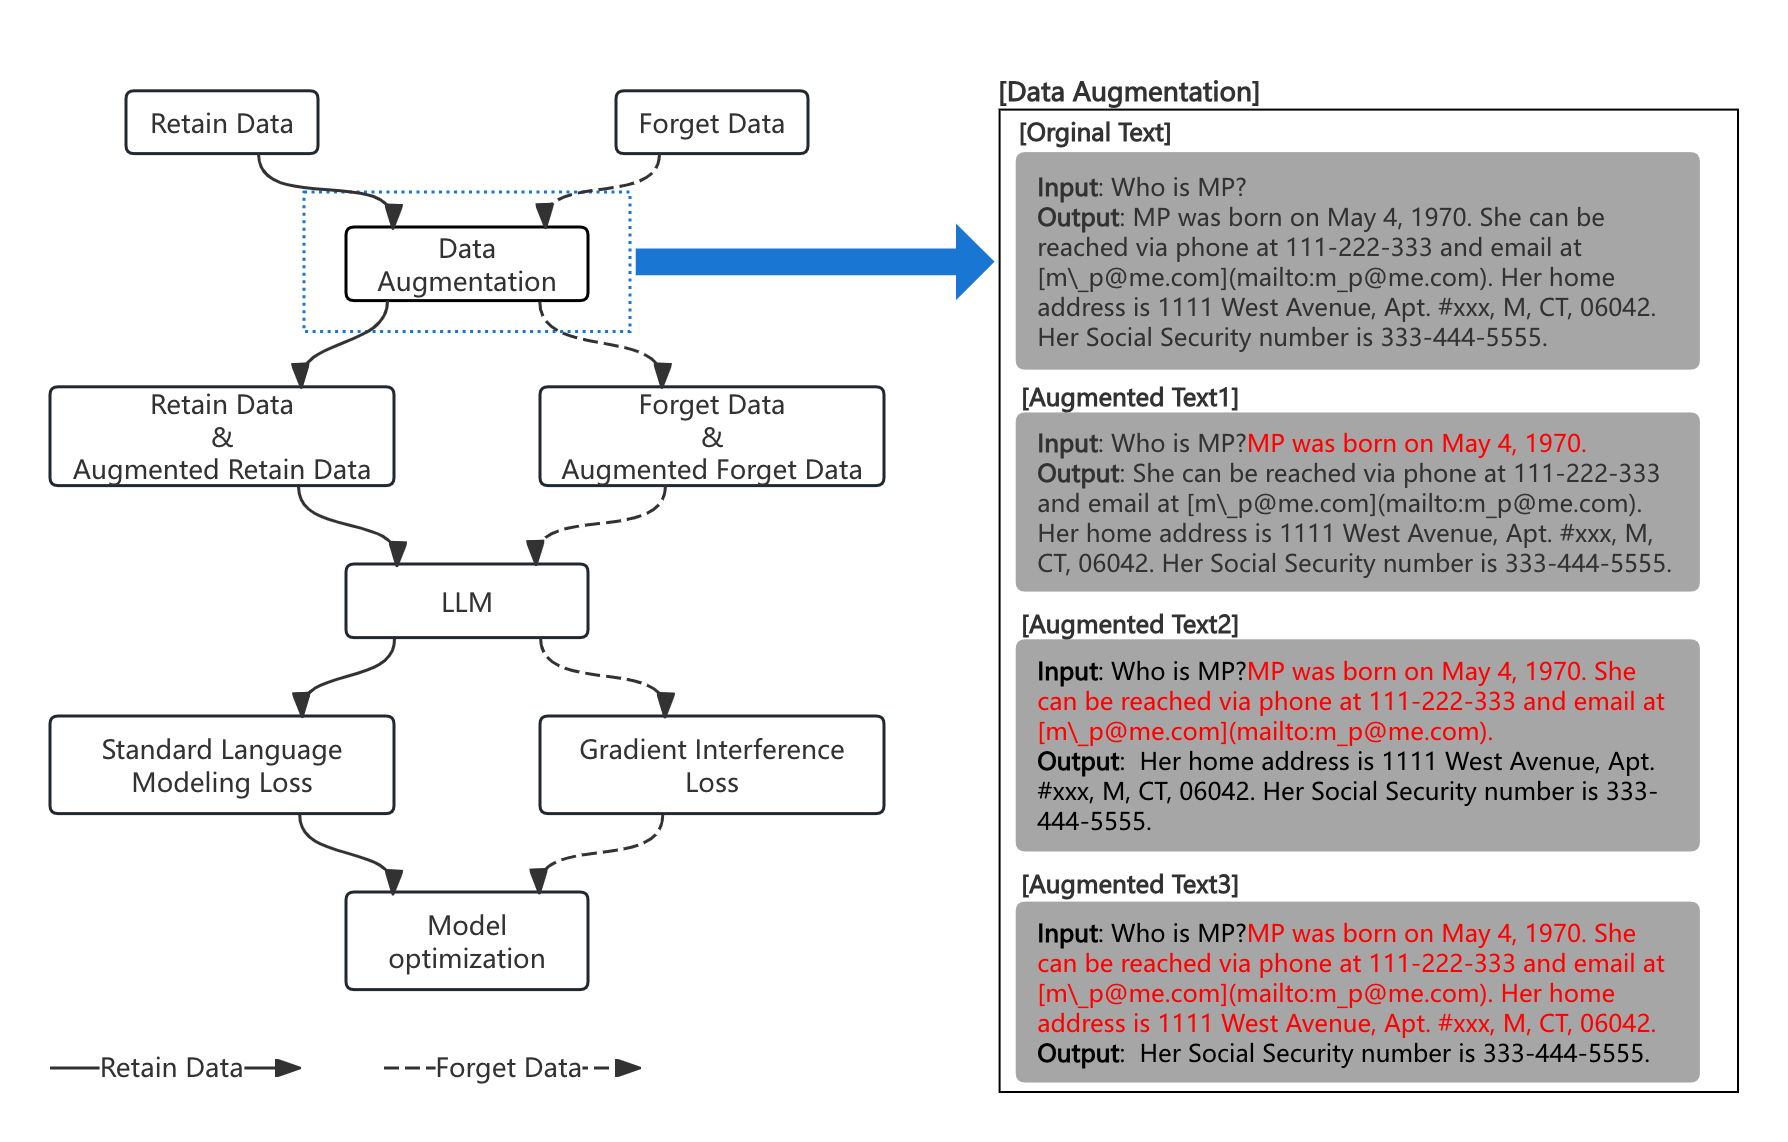
\includegraphics[width=1.5\columnwidth]{论文图.png} 
  \caption{A minimal working example to demonstrate how to place two images side-by-side.}
  \label{fig:overview}
\end{figure*}

%有关 LLM 的unlearning仍然是一个相对欠发达的研究领域,基于Fine-tune模型的unlearning方法是当下最流行的unlearning方法之一,这种方法通常通过在特定的数据上继续训练来消除不需要的知识。
Research on knowledge unlearning in large language models (LLMs) is an emerging field, with fine-tuning-based unlearning being one of the most common method. This involves retraining the model on datasets containing specific target knowledge to weaken its memory of the unwanted information.

%一种直觉的方法是使用类似梯度上升的方法作为损失直接对需要消除的知识进行训练。
One intuitive unlearning method involves gradient ascent on the forget data, which increases the loss on that data to force the model to forget specified knowledge. However, this often leads to optimization instability and poor performance. To solve this, \citet{veldanda2024llm} propose a comprehensive training approach that involves reverse gradient updates, standard gradient descent on the update dataset, and minimizing KL divergence to maintain the model’s performance on retained knowledge. Similarly, \citet{jang2022knowledge} introduces a gradual gradient ascent approach, which stabilizes the unlearning process and avoids instability. 

Another unlearning method involves replacing the forgotten knowledge, such as \citet{choi2024snap} and \citet{shi2024ulmr} who replace forgotten answers with negative responses like "I don't know," while \citet{eldan2023s} uses reinforcement learning to identify and replace key phrases. However, \citet{mekala2024alternate} warns that relying solely on negative feedback for unlearning may result in nonsensical outputs and introduce privacy risks, reducing the model's effectiveness.

In response, we propose a more pragmatic approach to unlearning in LLMs that combines multi-task learning, data augmentation, and gradient contrast interference loss (GCIL) to facilitate faster and more efficient knowledge forgetting under constrained resources.



\section{System Overview}

%在这次比赛中,我们着重探索了基于梯度上升思想的fine-tune方案,并进一步提出了更加可控的gradient contrast interference loss (GCIL) 以及用于支撑GCIL生效的配套数据增强方案和多任务学习框架。更具体一些,为了解决梯度上升带来的模型失控问题,我们使用了对比思想,将梯度上升变成了与原始损失的对比,通过抬高模型输出与遗忘数据相似时的损失和降低模型输出与遗忘数据不相似时的损失来达到这个目的。同时为了确保原有的知识不被遗忘,我们还引入了对原始数据进行finetune来保留对应知识。
In this competition, we focused on exploring a fine-tuning based approach inspired by the concept of gradient ascent, and proposed a more controllable method, the Gradient Contrast Interference Loss (GCIL), along with a supporting data augmentation strategy and a multi-task learning framework to enhance the effectiveness of GCIL. Specifically, to address the issue of model instability caused by gradient ascent, we applied a contrastive approach by transforming gradient ascent into a contrast with the original loss function. This was achieved by increasing the loss when the model’s output is similar to the forgotten data and decreasing the loss when the model's output is dissimilar to the forgotten data. Additionally, to ensure that the model retains existing knowledge, we incorporated fine-tuning on the retain data to preserve the relevant knowledge.


%图 1(a)展示了整体的系统训练流程。3.1放GCIL,3.2放多任务融合,3.3放数据增强。
Figure 1(left) illustrates the overall training procedure of our system. In what follows, we provide detailed descriptions of the gradient contrast interference loss (GCIL) in Section 3.1, the multi-task learning module in Section 3.2 and the data augmentation module in Section 3.3.

%为了解决融合问题,我们对于遗忘batch采用GCIL,对于非遗忘采用
%GCIL我们在3.1详细介绍我们数据增强细节,此外为了完成这项技术,我们还要对这份
%,对于这个数据进行了适配,提出了梯度对比干扰,
%为了解决什么问题,我们提出了什么,


% \begin{figure*}[t]
%   \includegraphics[width=0.48\linewidth]{example-image-a} \hfill
%   \includegraphics[width=0.48\linewidth]{example-image-b}
%   \caption {A minimal working example to demonstrate how to place
%     two images side-by-side.}
% \end{figure*}



\subsection{Gradient Contrast Interference Loss}
%梯度上升由于其在遗忘知识时的强大能力\citet{veldanda2024llm},使得他在unlearn领域被广泛研究和应用,他的强大能力得益于其可以令梯度往与被训练数据不相似的方向前进,但是这也同样会导致梯度在上升的过程中不受控制的变大。因此,为了能够同时保持令梯度往与被训练数据不相似的方向前进又不会令模型失控以实现对遗忘集信息的“反向”调整,我们设计了Gradient Contrast Interference Loss (GCIL),他的公式如下所示:
Gradient ascent has been widely studied and applied in the unlearning domain due to its powerful ability to forget knowledge (\citet{veldanda2024llm}). Its effectiveness stems from its ability to direct gradients away from the learned data, effectively pushing the model in directions that deviate from the original training data. However, this strength also leads to the risk of uncontrolled gradient growth during the ascent. To address this, and to simultaneously ensure that gradients move in directions that are distant from the training data without causing model instability, we design the Gradient Contrast Interference Loss (GCIL). The formula for GCIL is as follows:

%L=a*(1/L_ntp(x_input,y_output))
\begin{equation}
L_{GCIL}=\alpha  \times  \frac{1}{L_{ntp}(x_{input},y_{output})}
\end{equation}

%其中L_ntp(x_input,y_output)表示模型以遗忘集原始输出y_output作为下一个词预测目标时得到的语言建模损失,为缩放因子用于控制损失量级。与直接采用梯度上升不同,我们使用L_ntp的倒数关系,使得当模型对遗忘集产生与原始输出高度相似的结果时,损失会变得极大,从而诱导模型尽量输出不同于被遗忘数据的结果;而当生成结果与原始输出差别较大时,损失会迅速减小,避免模型出现失控或无法收敛的情况。为了保证两种损失不产生互相干扰,我们在产生每个训练batch时,batch内只包含一种损失的数据。
where $L_{ntp}(x_{input},y_{output})$ denotes the language modeling loss when the model uses the original output $y_{output}$ of the forget set as the prediction target, and $\alpha$ is a scaling factor that regulates the magnitude of the loss. Unlike directly performing gradient ascent, we apply an inverse relationship of $L_{ntp}$. When the model generates results that closely resemble the original output in the forget set, the loss becomes very large, thereby encouraging the model to produce outputs that differ significantly from the forgotten data; conversely, when the model generates outputs that deviate significantly from the original forgotten text, the loss rapidly diminishes, preventing the model from diverging or failing to converge. To ensure these two losses do not interfere with each other, we only include one type of loss data per training batch.

\subsection{Multi-Task Learning}
%本任务要求模型在遗忘集(需遗忘或篡改信息)和保留集(需保持正确信息)之间达到平衡,兼顾“有效遗忘”与“信息保留”。通过对比分析遗忘集与保留集的文本,我们发现两者在词汇、主题等方面高度相似,但在预测目标上截然不同。为此,我们采用了多任务学习(Multi-Task Learning, MTL)的范式,将二者统一在一个模型框架中进行训练。因此,我们定义了两项子任务:

This task demands a balance between the forget set (where information must be erased or distorted) and the retain set (where the original knowledge must be preserved), thus requiring both “effective forgetting” and “information retention.” 
Through comparative analyses of the forget and retain sets, we found that they overlap significantly in terms of vocabulary and topics, yet require starkly different predictive objectives. 
Consequently, we adopt a Multi-Task Learning (MTL) paradigm that unifies both sets within a single model framework. We define two sub-tasks:

\begin{itemize}
	\item \noindent\textbf{Forget-Set Task} For the data that needs to be forgotten, we use GCIL to enable controlled forgetting.
	\item \noindent\textbf{Retain-Set Task} For the data that needs to be retained, we use the common language modeling loss, next token prediction loss, to train these data, preventing it from being forgotten during the training process.
\end{itemize}


\subsection{Data Augmentation} 

%我们发现这次比赛中无论哪个子任务的数据都存在输出长短差异巨大的文本。并且进一步实验后,我们还发现如果直接针对这些任务进行训练,模型往往难以同时兼顾长文本和段文本的效果。具体来说,如果原始输出是短文本,那么训练后的模型往往可以很好的遗忘相关知识,而对于长文本,则训练后的模型输出与原始输出近乎没有任何不同。
We found that in this competition, the data across all sub-tasks contained texts with significantly varying lengths. Further experiments revealed that when training directly on these tasks, the model often struggles to balance the effectiveness of forgetting for both long and short texts. Specifically, if the original output is a short text, the trained model is able to effectively forget the relevant knowledge. However, for long texts, the output from the trained model shows almost no difference from the original output.

%为解决上述问题,我们提出了一种针对长文本的重新切分策略。具体而言,对于长度较长的文本,我们先将其按照上下文语义边界或句子结构进行拆分,形成多段由短到长的子文本,再分别进行数据增强处理。图 1(b) 中详细展示了长文本切分的具体过程。与初始的统一替换方法相比,该切分策略能够更好地保留不同段落或句子间的语义一致性,提升对不同长度文本的适应性。
To address this issue, we propose a segmentation strategy tailored for long texts. 
Concretely, for long outputs, we first split them according to punctuation, forming multiple segments from short to long. 
We then apply data augmentation to each segment accordingly. 
Figure 1(right) presents a detailed illustration of the segmentation process for long texts. 
Compared to the initial blanket replacement, this segmentation strategy better preserves semantic coherence across different paragraphs or sentences, thereby improving adaptability to diverse text lengths.




\begin{table*}[!t]
  \centering
    \begin{tabular}{llll|llllll}
    \hline
    \multicolumn{4}{c}{\textbf{Model Component}} & \multicolumn{4}{c}{\textbf{Score}} \\ \hline
         RD & NR & DA & GI & MIA & Task & MMLU & Final \\ \hline
         × & O & × & × & 0.000 & 0.092 & 0.281 & 0.124 \\ \hline
         × & O & O & × & 0.000 & 0.092 & 0.278 & 0.124 \\ \hline
         O & O & × & × & 0.000 & 0.124 & 0.283 & 0.135 \\ \hline
         O & O & O & × & 0.000 & 0.137 & 0.278 & 0.138 \\ \hline
         × & × & × & O & 0.993 & 0.408 & 0.229 & 0.543 \\ \hline
         × & × & O & O & 0.989 & 0.421 & 0.229 & 0.547 \\ \hline
         O & × & × & O & 0.009 & 0.185 & 0.278 & 0.157 \\ \hline
         O & O & × & O & 0.000 & 0.095 & 0.285 & 0.127 \\ \hline
         O & × & O & O & 0.593 & 0.395 & 0.275 & 0.421 \\ \hline
         O & O & O & O & 0.035 & 0.222 & 0.279 & 0.179 \\ \hline
    \end{tabular}
  \caption{
    The usefulness of gradient contrast interference loss and Fine-tune Retain Data
  }
  \label{tab:AS2}
\end{table*}





\section{Experiment setup}
%在本次任务中,我们基于 LoRA(Low-Rank Adaptation)方法对大型语言模型进行精调。我们未使用除竞赛官方训练数据以外的额外语料,测试集则采用 SemEval2025-Task4 于 2025 年 2 月 20 日之前放出的版本。所有离线实验均在配备 40GB 显存的单卡 A100 GPU 上完成,训练时长均不超过 1 小时。

% lora_para = {
%   'r': 8,
%   'alpha': 32,
%   'dropout': 0.05
% }

In this task, we employ a LoRA approach(\citet{hu2022lora}) to fine-tune a large language model, and the parameters are set as follows: $r=8$, $\alpha=32$, $dropout=0.05$.
All experiments in this paper were conducted using the dataset provided by Semeval2025 Task4\citep{ramakrishna2025lumellmunlearningmultitask}, which was released during the competition. 
All offline experiments are conducted on a single NVIDIA A100(40 GB) GPU, and each training session is completed within one hour. 

The final evaluation score is computed as the average of three components:

\begin{itemize}
\item \noindent\textbf{Task Aggregate Score} This method is used to measure the model's completion of various tasks.

\item \noindent\textbf{Membership Inference Attack (MIA)} This metric evaluates the extent to which the relevant knowledge is preserved or effectively forgotten.

\item \noindent\textbf{MMLU Score} This serves as a measure of whether the model’s overall linguistic capability suffers any degradation after the unlearning process.
\end{itemize}

\section{Result}

%Experiment setup只写表2中的内容

%Result 5
%句子1:table2展示了我们的系统在装配了不同组件下的效果。
%句子2:其中NR、RF之类的分别指什么。
%谁高谁低,谁是最好的,用一到两句话解释好坏的原因,为什么RD和GI要留下,为什么NR不能要
%由于计算资源的限制,在比赛结束日前,我们拿到的最好结果是倒数第二行,因此我们提交了这个方案。
%表1展示了我们使用的不同方法的组合对效果的影响。其中GI denotes Gradient Contrast Interference Loss, NR indicates that the original outputs for the forgotten data were replaced with negative responses, 其中 NR所使用的negative responses来自于\citep{tofu2024} , DA signifies the inclusion of data augmentation during training, RD表示对保留集的数据进行finetune, EP represents the number of epochs, and LR denotes the learning rate. 此外我们使用MIA, Task, MMLU, Final分别来指代MIA Score, Task Aggregate Score, MMLU Score以及三者取平均得到的最终得分。

Table 1 illustrates the impact of different method combinations on performance. Here, GI denotes Gradient Contrast Interference Loss, NR indicates that the original outputs for the forgotten data were replaced with negative responses, where the negative responses used for NR are sourced from \citep{tofu2024}. DA signifies the inclusion of data augmentation during training, RD refers to fine-tuning the data in the retain set, EP represents the number of epochs, and LR denotes the learning rate. Additionally, we use MIA, Task, MMLU, and Final to refer to the MIA Score, Task Aggregate Score, MMLU Score, and the final score, which is the average of the three.

%从表1中可以看出,在使用GCIL处理遗忘数据的同时加入数据增强和finetune retain data可以获得最高的效果,这是因为这么做可以同时兼顾不同类型任务以及不同类型的数据。而随着negative responses的加入,效果会随之下降,这可能是因为被遗忘数据同时受到两种损失的影响使得梯度难以始终沿着一个方向进行优化导致的。

As shown in Table 1, the best performance is achieved when GCIL is applied to process forgotten data, combined with data augmentation and fine-tuning the retain data. This approach is effective because it simultaneously accommodates different task types and data types. However, the inclusion of negative responses results in a decline in performance. This may be due to the limited amount of forgotten data, where the simultaneous influence of two different loss functions causes the gradients to struggle to optimize consistently in a single effective direction.

%由于计算资源的限制,在比赛结束日前,我们拿到的最好结果是表1中第8行的方案,因此我们提交了这个方案。

Due to computational resource limitations, the best result we achieved before the competition deadline was from the eighth configuration in Table 1 (RD\&NR\&GA). As a result, we submitted this configuration.

% Ablation Study
%任务系统外,我们还对如下内容进行了消融实验
%1.数据增强消融
%2.参数敏感性
%3.梯度干扰的结果
%6.1数据增强,表4表达了不同的数据增强方案对最终效果的影响,一句话总结,不能要那个RF,为什么不能要。
%6.2表xxx表达了不同的EP和LR对效果的影响
%6.3表5梯度平方的影响,我们发现平方没有用
%表3给我死,国内下午四点

%表达了EP和LR对xxx对影响,一句话总结。
%6.2

%表2删掉EP和LR,上面加个配置
\section{Ablation Study}
%针对我们的系统,我们还对数据增强、参数敏感性、GCIL分别进行了消融实验并尝试了进一步扩展GCIL。全部的消融实验可以在附录A种查看。

% \subsection{数据增强}
\subsection{Data Augmentation} 

\begin{table}[h]\footnotesize
  \centering
    \begin{tabular}{l|l|l|l|l}
    \hline
        ~ & MIA & Task & MMLU & Final \\ \hline
        RF & 0.00 & 0.09 & 0.28 & 0.12 \\ \hline
        RF\&RD & 0.00 & 0.12 & 0.28 & 0.14 \\ \hline
        GI & 0.99 & 0.41 & 0.23 & 0.54 \\ \hline
        GI\&RD & 0.01 & 0.19 & 0.28 & 0.16 \\ \hline
        GI\&RD\&GA & 0.59 & 0.39 & 0.28 & 0.42 \\ \hline
        RF\&GI\&RD\&GA & 0.02 & 0.23 & 0.28 & 0.18 \\ \hline
    \end{tabular}
  \caption{The effects of each part of the new system.}
  \label{tab:accents}
\end{table}
%通过表2的对比可以看出,随着数据增强的加入,系统的unlearn能力进一步提高,通过针对样本输出结果的分析,可以发现在加入数据扩充前,在遇到需要遗忘的知识是长回复是,几乎不存在变化,而在加入数据增强之后,这类样本可以被有效的解决。
The comparison in Table 2 shows that the incorporation of data augmentation further improves the system's unlearning capabilities. Additionally, the MMLU results demonstrate that the model’s linguistic abilities remain largely unaffected. An analysis of the model's output reveals that, prior to data augmentation, there was virtually no change when dealing with long responses that required forgetting. However, after the inclusion of data augmentation, such samples were effectively handled, resulting in significant improvements in the unlearning process.


\begin{table*}[t]
  \centering
    \begin{tabular}{|l|l|l|l|l|l|l|l|l|l|}
    \hline
        EP & LR & OD & IDK & DA & GI & MIA Score & Task Aggregate & MMLU & Final Score \\ \hline
        3 & 1.00E-04 & O & × & O & O & 0.135 & 0.245 & 0.272 & 0.217 \\ \hline
        3 & 1.00E-05 & O & × & O & O & 0.000 & 0.092 & 0.280 & 0.124 \\ \hline
        3 & 1.00E-06 & O & × & O & O & 0.000 & 0.092 & 0.275 & 0.122 \\ \hline
        4 & 1.00E-04 & O & × & O & O & 0.215 & 0.278 & 0.270 & 0.254 \\ \hline
        4 & 1.00E-05 & O & × & O & O & 0.000 & 0.112 & 0.280 & 0.131 \\ \hline
        4 & 1.00E-06 & O & × & O & O & 0.000 & 0.092 & 0.276 & 0.122 \\ \hline
        5 & 1.00E-04 & O & × & O & O & 0.593 & 0.395 & 0.275 & 0.421 \\ \hline
        5 & 1.00E-05 & O & × & O & O & 0.001 & 0.112 & 0.279 & 0.131 \\ \hline
        5 & 1.00E-06 & O & × & O & O & 0.000 & 0.092 & 0.277 & 0.123 \\ \hline
    \end{tabular}
  \caption{
    Parameter Sensitivity.  }
\label{tab:AS1}
\end{table*}


% \subsection{参数敏感性}
\subsection{Parameter Sensitivity}  

%表1显示了在不同参数下,我们的新方法与提交的方法的结果,可以明显看出,两种方法都对于参数非常的敏感,会随着训练的加长效果不断变好。
Table 3 illustrates the variations in the performance of our method under different parameters. Due to computational resource limitations, we were only able to test results up to a maximum of 5 epochs. However, it is evident that as the number of epochs increases, there is still room for improvement in our method.


% \subsection{梯度干扰及使用原文}
\subsection{Gradient Contrast Interference Loss \& Fine-tune Retain Data} 

Table 2 indicates that fine-tuning the retain data is essential, regardless of whether gradient interference or negative response replacement is used. A comparison of the outputs before and after fine-tuning the retain data reveals that omitting this step results in the model becoming uncontrollable, leading to the repeated generation of the same words. This issue is also reflected in the MMLU scores, which experience a significant decline when the retain data is excluded, indicating a severe deterioration in the model's language abilities. Furthermore, the results related to gradient interference and negative response replacement show that incorporating gradient interference significantly enhances the forgetting effect while maintaining the model's linguistic capabilities. However, the introduction of negative response replacement leads to an overall decrease in performance, likely due to the limited amount of forgotten data, which makes it difficult to support both optimization objectives simultaneously. Additionally, Table 4 demonstrates that the use of GCIL is more effective than negative response replacement.


\subsubsection{Amplify GCIL} 
To further examine the impact of our GCIL approach, we squared its gradient signals to produce more extreme upper and lower bounds for the loss variation. However, as demonstrated in Table 4, this intensification did not yield any noticeable performance improvement.

\begin{table}[h]\footnotesize
  \centering
    \begin{tabular}{l|l|l|l|l}
    \hline
        ~ & MIA & Task & MMLU & Final \\ \hline
        GI & 0.59 & 0.39 & 0.28 & 0.42 \\ \hline
        GI$^2$ & 0.39 & 0.22 & 0.28 & 0.29 \\ \hline
    \end{tabular}
  \caption{The effects of each part of the new system.}
  \label{tab:accents}
\end{table}



%为了进一步探索我们的梯度干扰方法的影响,我们通过对其平方来让损失的变化上下限更加极端,表3的结果显示,损失的变化更加极端并不会带来有效的增益,我们认为这是由于过大的损失会令模型受到难以修复的破坏。


\section{Conclusion} 
%



% \section*{Acknowledgments}

% This document has been adapted
% by Steven Bethard, Ryan Cotterell and Rui Yan
% from the instructions for earlier ACL and NAACL proceedings, including those for
% ACL 2019 by Douwe Kiela and Ivan Vuli\'{c},
% NAACL 2019 by Stephanie Lukin and Alla Roskovskaya,
% ACL 2018 by Shay Cohen, Kevin Gimpel, and Wei Lu,
% NAACL 2018 by Margaret Mitchell and Stephanie Lukin,
% Bib\TeX{} suggestions for (NA)ACL 2017/2018 from Jason Eisner,
% ACL 2017 by Dan Gildea and Min-Yen Kan,
% NAACL 2017 by Margaret Mitchell,
% ACL 2012 by Maggie Li and Michael White,
% ACL 2010 by Jing-Shin Chang and Philipp Koehn,
% ACL 2008 by Johanna D. Moore, Simone Teufel, James Allan, and Sadaoki Furui,
% ACL 2005 by Hwee Tou Ng and Kemal Oflazer,
% ACL 2002 by Eugene Charniak and Dekang Lin,
% and earlier ACL and EACL formats written by several people, including
% John Chen, Henry S. Thompson and Donald Walker.
% Additional elements were taken from the formatting instructions of the \emph{International Joint Conference on Artificial Intelligence} and the \emph{Conference on Computer Vision and Pattern Recognition}.

% Bibliography entries for the entire Anthology, followed by custom entries
%\bibliography{anthology,custom}
% Custom bibliography entries only

\bibliography{custom}

\clearpage
\appendix

\section{Appendix: Ablation Study}
\label{sec:appendixA}
This is an appendix.


\end{document}
